\newpage
\section{Auswertung}     


\begin{table}[H]
    \centering
    \begin{tabular}{S [table-format=3.0] S [table-format=3.0] S [table-format=5.0]S [table-format=5.0]}
        \toprule
        {$U \mathbin{\scalebox{1.5} / }\si{\volt}$} & {$U \mathbin{\scalebox{1.5} / }\si{\volt}$} & {$N \mathbin{\scalebox{1.5} / }\si{\per\second}$}  & {$N \mathbin{\scalebox{1.5} / }\si{\per\second}$}\\
        \midrule
        320 & 520 & 9672  & 10255 \\ 
        330 & 530 & 9689  & 10151 \\
        340 & 540 & 9580  & 10351 \\
        350 & 550 & 9837  & 10184 \\
        360 & 560 & 9886  & 10137 \\
        370 & 570 & 1004  & 10186 \\
        380 & 580 & 9996  & 10171 \\
        390 & 590 & 9943  & 10171 \\
        400 & 600 & 9995  & 10253 \\
        410 & 610 & 9980  & 10368 \\
        420 & 620 & 9986  & 10365 \\
        430 & 630 & 9960  & 10224 \\
        440 & 640 & 10219 & 10338 \\
        450 & 650 & 10264 & 10493 \\
        460 & 660 & 10174 & 10467 \\
        470 & 670 & 10035 & 10640 \\
        480 & 680 & 10350 & 10939 \\
        490 & 690 & 10290 & 11159 \\
        500 & 700 & 10151 & 11547 \\
        510 & /   & 10110 &  /    \\
        \bottomrule
    \end{tabular}
\caption{Die Messwerte der Spannung gegen die Anzahl der Impulse pro 60/s.}
\label{tab:Uamp}
\end{table}

Die Daten werden in ein Diagramm eingezeichnet und mit einem Fehlerbalken versehen. Der Fehler entspricht der Wurzel der Anzahl der Impulse.
Durch das Plateau wird eine Ausgleichsgerade der Form $y = mx + b$ gelegt. Die Werte für die Ausgleichsgerade ergeben sich zu:
\begin{align}
    m&= \num{1.138 \pm 0.24} \nonumber \\
    b&= \num{959 \pm 121}    \nonumber
\end{align}

\begin{figure}[H]
    \centering
    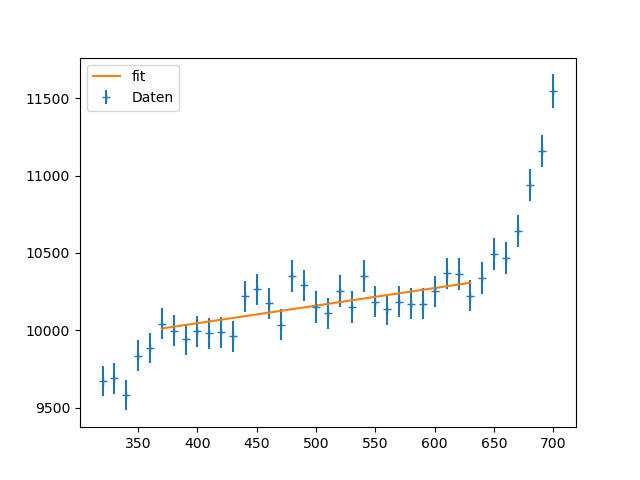
\includegraphics[width=0.85\textwidth]{build/plots/a.png}
    \caption{Die Charasteristik des Zählrohrs mit linearem fit auf dem Plateau.}
    \label{img:plot1}
\end{figure}


